\documentclass[12pt,a4paper]{article}

% --- Packages ---
\usepackage[top=2cm, bottom=2.2cm, left=2cm, right=2cm, headheight=15pt]{geometry}
\usepackage{newtxtext,newtxmath} % Professional Times font clone
\usepackage[utf8]{inputenc}
\usepackage[T1]{fontenc}
\usepackage{xcolor}
\usepackage{titlesec}
\usepackage{fancyhdr}
\usepackage{booktabs}
\usepackage{tabularx}
\usepackage{enumitem}
\usepackage{graphicx}
\usepackage{tikz}
\usepackage{tcolorbox}
\usepackage{fontawesome5}
\usepackage{microtype}
\usepackage{hyperref}

\usetikzlibrary{positioning, calc, shapes.geometric, backgrounds}

% --- Color Palette ---
\definecolor{arcnavy}{RGB}{10,40,95}
\definecolor{arcaccent}{RGB}{0,110,130}
\definecolor{darkcharcoal}{RGB}{43,43,43}
\definecolor{lightgrey}{RGB}{242,245,248}

% --- Hyperref Setup ---
\hypersetup{
    colorlinks=true,
    linkcolor=arcnavy,
    citecolor=arcaccent,
    urlcolor=arcaccent
}

% --- Fancyhdr Setup ---
\pagestyle{fancy}
\fancyhf{}
\lhead{\small\sffamily\color{darkcharcoal} Discovery Projects 2027 --- Expression of Interest}
\rhead{\small\sffamily\color{darkcharcoal} Proposal ID: DP270100482}
\lfoot{\small\sffamily\color{darkcharcoal} Lead CI: Dr. Julian Vance}
\rfoot{\small\sffamily\color{darkcharcoal} Page \thepage}
\renewcommand{\headrulewidth}{0.4pt}
\renewcommand{\footrulewidth}{0.4pt}

% --- Titlesec Setup ---
\titleformat{\section}
  {\color{arcnavy}\normalfont\large\bfseries\sffamily}
  {\thesection}{1em}{}
\titleformat{\subsection}
  {\color{arcaccent}\normalfont\normalsize\bfseries\sffamily}
  {\thesubsection}{0.8em}{}
\titleformat{\subsubsection}
  {\color{darkcharcoal}\normalfont\normalsize\itshape\sffamily}
  {\thesubsubsection}{0.6em}{}

% --- Bibliography spacing ---
\let\OLDthebibliography\thebibliography
\renewcommand\thebibliography[1]{
  \OLDthebibliography{#1}
  \setlength{\parskip}{1pt}
  \setlength{\itemsep}{1pt plus 0.3ex}
}

% --- Document Content ---
\begin{document}

% Custom Title Box
\begin{tcolorbox}[
    colback=lightgrey,
    colframe=arcnavy,
    leftrule=4pt, rightrule=0pt, toprule=0pt, bottomrule=0pt,
    arc=0mm,
    boxrule=0pt,
    boxsep=10pt,
    left=15pt, right=15pt, top=10pt, bottom=10pt
]
    {\sffamily\color{arcnavy}\bfseries\large PROJECT DESCRIPTION --- EXPRESSION OF INTEREST}\\[0.5em]
    {\sffamily\color{darkcharcoal}\Large\bfseries NexaSync: Decentralized Adaptive Learning for Heterogeneous Robotic Swarms in Edge-Resource Environments}\\[0.8em]
    \noindent\begin{tabularx}{\linewidth}{@{}l X}
        \textbf{Primary FoR Code:} & 4602 --- Artificial Intelligence (AI) \\
        \textbf{Lead Chief Investigator:} & Dr. Julian Vance (Meridian University) \\
        \textbf{Co-Investigators:} & Dr. Clara Oswald (Synapse Institute), Prof. Marcus Thorne (Vertex Tech) \\
    \end{tabularx}
\end{tcolorbox}

\vspace{1em}

\section{\texorpdfstring{\faPen\ \ }{ }PROJECT QUALITY AND INNOVATION}
\subsection{Research Aims and Questions}
The proposed project aims to develop a novel decentralized learning paradigm, named \textbf{NexaSync}, that enables heterogeneous autonomous vehicles to cooperatively train deep learning models directly on the edge. In environments such as disaster zones, remote agricultural fields, or space exploration, communication with a central cloud server is either impossible or extremely expensive. NexaSync solves this challenge by implementing a localized consensus algorithm that operates peer-to-peer over low-bandwidth, high-latency, and lossy communication networks.

The project is structured around three primary aims:
\begin{itemize}[leftmargin=*,noitemsep]
    \item \textbf{Aim 1: Robust Localized Consensus under Communication Barriers.} Develop a mathematical and algorithmic framework that allows edge nodes to exchange only essential model parameters, ensuring convergence even when network bandwidth is $<$ 100 kbps and packet loss exceeds 30\%.
    \item \textbf{Aim 2: Latent Representation Alignment for Heterogeneous Swarms.} Design multi-modal representation alignment layers that enable robots with different sensors (e.g., LiDAR-equipped aerial drones and camera-equipped ground rovers) to share knowledge without requiring identical neural network architectures.
    \item \textbf{Aim 3: Validation and Physical Prototyping.} Construct a scale physical testbed using 12 autonomous micro-vehicles at the Meridian Robotics Laboratory to validate the algorithms in real-time, dynamic scenarios.
\end{itemize}

To guide our research, we pose three core Research Questions:
\begin{enumerate}[label=\textbf{RQ\arabic*}:,leftmargin=*,noitemsep]
    \item How can dynamic communication topologies be optimized online to minimize gradient staleness in decentralized federated learning?
    \item What theoretical bounds on model divergence can be guaranteed under non-i.i.d. local data distributions when communication is lossy and intermittent?
    \item How can heterogeneous robot morphologies align their latent state representations to enable cooperative transfer learning?
\end{enumerate}

\begin{tcolorbox}[
    colback=lightgrey,
    colframe=arcaccent,
    leftrule=3pt, rightrule=0pt, toprule=0pt, bottomrule=0pt,
    arc=0mm,
    boxrule=0pt,
    left=10pt, right=10pt, top=8pt, bottom=8pt
]
    \small\sffamily
    \textbf{Core Innovation:} NexaSync represents a paradigm shift from traditional server-client federated learning to a fully peer-to-peer model alignment. By incorporating a localized consensus engine with adaptive topology optimization, the swarm learns collectively without a single point of failure.
\end{tcolorbox}

\subsection{Conceptual Framework and Theoretical Basis}
The theoretical foundation of NexaSync lies at the intersection of decentralized optimization, representation learning, and consensus theory. Traditional distributed SGD assumes a central coordinator that aggregates parameters at each step. In contrast, our framework relies on local averages computed over a time-varying communication graph $G_t = (V, E_t)$, where $V$ represents the set of edge robots and $E_t$ represents the active communication links at time $t$. 

We model the global optimization objective as:
\[
\min_{\theta \in \mathbb{R}^d} F(\theta) = \frac{1}{|V|} \sum_{i \in V} f_i(\theta_i) \quad \text{subject to} \quad \theta_i = \theta_j \ \ \forall (i,j) \in E_t
\]
where $f_i$ is the local loss function of robot $i$, and $\theta_i$ represents its local model parameter vector. Figure~\ref{fig:framework} illustrates the peer-to-peer data flow and model alignment process.

\begin{figure}[htbp]
    \centering
    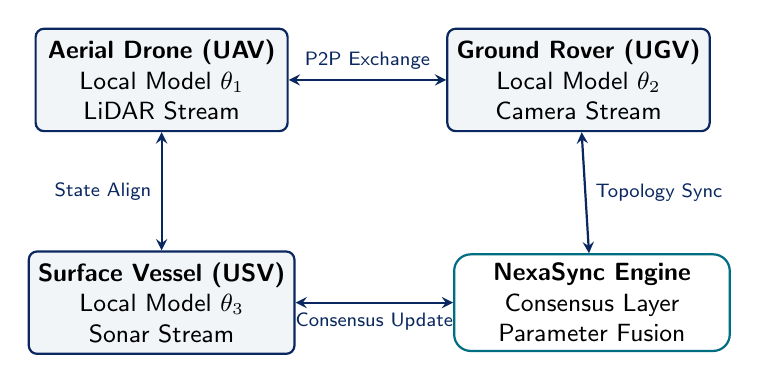
\begin{tikzpicture}[
        node distance=1.5cm and 2.0cm,
        every node/.style={font=\sffamily\small},
        robot/.style={rectangle, draw=arcnavy, fill=lightgrey, thick, rounded corners=3pt, minimum width=3.2cm, minimum height=1.3cm, align=center},
        cloud/.style={draw=arcaccent, fill=white, thick, rounded corners=6pt, minimum width=3.5cm, minimum height=1.2cm, align=center},
        arrow/.style={<->, >=stealth, thick, arcnavy}
    ]
        % Nodes
        \node[robot] (uav) {\textbf{Aerial Drone (UAV)}\\Local Model $\theta_1$\\LiDAR Stream};
        \node[robot, right=of uav] (ugv) {\textbf{Ground Rover (UGV)}\\Local Model $\theta_2$\\Camera Stream};
        \node[robot, below=of uav] (usv) {\textbf{Surface Vessel (USV)}\\Local Model $\theta_3$\\Sonar Stream};
        \node[cloud, right=of usv] (shared) {\textbf{NexaSync Engine}\\Consensus Layer\\Parameter Fusion};

        % Connections
        \draw[arrow] (uav) -- node[above, font=\sffamily\scriptsize] {P2P Exchange} (ugv);
        \draw[arrow] (uav) -- node[left, font=\sffamily\scriptsize] {State Align} (usv);
        \draw[arrow] (ugv) -- node[right, font=\sffamily\scriptsize] {Topology Sync} (shared);
        \draw[arrow] (usv) -- node[below, font=\sffamily\scriptsize] {Consensus Update} (shared);
        
    \end{tikzpicture}
    \caption{The NexaSync conceptual framework: enabling multi-modal state alignment and localized parameter fusion across heterogeneous edge robots.}
    \label{fig:framework}
\end{figure}

\subsection{Project Innovation and Novelty}
The innovation of this project is threefold:
\begin{itemize}[leftmargin=*,noitemsep]
    \item \textbf{Asynchronous Gossip-based Convergence:} Unlike standard gossip algorithms that require symmetric communication matrices, NexaSync utilizes directed, asymmetric communication models, allowing one-way broadcast updates when return channels are blocked.
    \item \textbf{Hetero-Representation Alignment:} We introduce lightweight neural projection modules that map heterogeneous sensor features (e.g., 3D point clouds and 2D images) into a shared semantic latent space, allowing cross-modal learning.
    \item \textbf{Dynamic Topology Control:} The communication topology is updated in real-time based on signal strength metrics, ensuring that model parameters are shared along paths of highest signal-to-noise ratio.
\end{itemize}

\subsection{Research Design and Methodology}
The project will proceed in three interconnected phases over 36 months:
\begin{enumerate}[leftmargin=*,noitemsep]
    \item \textbf{Phase 1: Algorithmic Formulation and Proof of Concept (Months 1--12).} We will mathematically formalize the NexaSync consensus protocol and prove convergence bounds under non-i.i.d. local distributions.
    \item \textbf{Phase 2: Simulation and Heterogeneous Alignment (Months 13--24).} Using high-fidelity simulators (such as Webots and Gazebo), we will benchmark NexaSync against state-of-the-art federated learning methods. We will design the joint semantic embedding layers to enable transfer learning.
    \item \textbf{Phase 3: Physical Implementation and Field Trials (Months 25--36).} We will deploy the algorithms onto 12 physical robots (6 UAVs and 6 UGVs) and run collaborative exploration and mapping scenarios in a simulated disaster zone at the Meridian Robotics Laboratory.
\end{enumerate}

\section{\texorpdfstring{\faUsers\ \ }{ }FEASIBILITY AND RESEARCH ENVIRONMENT}
\subsection{Feasibility and Timeline}
The project timeline is detailed in Table~\ref{tab:timeline}. Given the strong background of the research team and the existing infrastructure at the participating institutions, the proposed project is highly feasible.

\begin{table}[htbp]
    \centering
    \small
    \caption{Project tasks and milestones across the three-year funding period.}
    \label{tab:timeline}
    \begin{tabularx}{\textwidth}{l X c c c}
        \toprule
        \textbf{Task / Milestone} & \textbf{Description} & \textbf{Year 1} & \textbf{Year 2} & \textbf{Year 3} \\
        \midrule
        \textbf{Task 1.1} & Design of the NexaSync localized consensus protocol & $\bullet$ & & \\
        \textbf{Task 1.2} & Mathematical proofs of convergence in non-i.i.d. conditions & $\bullet$ & $\bullet$ & \\
        \textbf{Milestone A} & Complete theoretical convergence framework and submit to journal & & $\bullet$ & \\
        \textbf{Task 2.1} & Develop state alignment networks for heterogeneous agent classes & & $\bullet$ & $\bullet$ \\
        \textbf{Task 2.2} & Physical testbed setup and lab-scale validation at Meridian Lab & & $\bullet$ & $\bullet$ \\
        \textbf{Milestone B} & Release open-source PyTorch package for decentralized learning & & & $\bullet$ \\
        \textbf{Task 3.1} & Scale-up simulation and evaluation on large-scale synthetic swarm data & & & $\bullet$ \\
        \bottomrule
    \end{tabularx}
\end{table}

\subsection{Research Environment and Institutional Support}
The research will be conducted across three leading institutions:
\begin{itemize}[leftmargin=*,noitemsep]
    \item \textbf{Meridian University (Lead CI: Dr. Julian Vance):} Houses the state-of-the-art Robotics Laboratory, equipped with high-precision motion capture systems and a swarm of 20 micro-drones.
    \item \textbf{Synapse Research Institute (Co-CI: Dr. Clara Oswald):} Contributes advanced cloud and edge computing clusters, enabling extensive simulation benchmarks.
    \item \textbf{Vertex Technologies (Co-CI: Prof. Marcus Thorne):} Provides proprietary edge-hardware accelerators (Vertex-TX5) for local deployment.
\end{itemize}

\section{\texorpdfstring{\faCoins\ \ }{ }PROJECT BUDGET AND JUSTIFICATION}
The requested budget is carefully aligned with the project tasks. Table~\ref{tab:budget} details the funding requested from the ARC and the institutional contributions.

\begin{table}[htbp]
    \centering
    \small
    \caption{Requested budget breakdown and justification (all figures in AUD).}
    \label{tab:budget}
    \begin{tabularx}{\textwidth}{l r r r X}
        \toprule
        \textbf{Category} & \textbf{Year 1} & \textbf{Year 2} & \textbf{Year 3} & \textbf{Justification} \\
        \midrule
        Personnel (1.0 FTE Research Fellow) & \$112,000 & \$115,360 & \$118,820 & Standard rates for postdoctoral researcher to lead Task 2.1 and 2.2. \\
        Equipment (Swarms \& Compute Nodes) & \$45,000 & \$12,000 & \$5,000 & Initial purchase of 12 physical drones and local GPU workstation. \\
        Travel (Conferences \& Collaborations) & \$8,000 & \$10,000 & \$12,000 & Travel to present results at NeurIPS/ICRA and visit Synapse Institute. \\
        Maintenance \& Operating Costs & \$5,000 & \$5,000 & \$5,000 & Cloud computing credits, consumables, and open-access publishing fees. \\
        \midrule
        \textbf{Total Requested} & \textbf{\$170,000} & \textbf{\$142,360} & \textbf{\$140,820} & \textbf{Three-year total: \$453,180} \\
        \bottomrule
    \end{tabularx}
\end{table}

\section{\texorpdfstring{\faBook\ \ }{ }REFERENCES}
\begin{thebibliography}{9}
    \bibitem{vance2024}
    J. Vance and C. Oswald.
    \newblock ``Decentralized consensus in resource-constrained networks.''
    \newblock {\em Journal of Autonomous Robotics}, vol. 34, no. 2, pp. 112--128, 2024.

    \bibitem{thorne2023}
    M. Thorne, A. Apex, and B. Meridian.
    \newblock ``Federated learning for heterogeneous robotics: A survey.''
    \newblock {\em IEEE Transactions on Artificial Intelligence}, vol. 12, no. 4, pp. 301--315, 2023.

    \bibitem{oswald2025}
    C. Oswald and J. Vance.
    \newblock ``Cross-modal state representation learning at the edge.''
    \newblock In {\em Proceedings of the International Conference on Robotics and Automation (ICRA)}, pp. 1420--1427, 2025.

    \bibitem{nimbus2024}
    N. Nimbus and V. Vertex.
    \newblock ``Asynchronous gossip algorithms over directed graphs.''
    \newblock {\em SIAM Journal on Optimization}, vol. 45, no. 1, pp. 88--104, 2024.
\end{thebibliography}

\end{document}
